\documentclass{article}
\usepackage{multicol}
\usepackage{xcolor}
\usepackage{graphicx}
\linespread{1.35}
\usepackage{amsmath}
\usepackage{color}
\usepackage{tikz}
\usetikzlibrary{arrows,automata}


\begin{document}


\begin{flushright}
 \texttt{Finite Automata} \hspace*{1cm} \textbf{49}
\end{flushright}

\vspace*{0.2cm}
\begin{multicols}{2}
\textbf{Definition:} An automaton is a system where materials,
energy, or information are transformed and transmitted
for performing some operation without the direct
participation of a human.\\
\hspace*{0.5cm} Any automated machine can be given as an example
of automaton. A model of finite automata is given in
Fig. 3.1.\\

\vspace*{0.2cm}
\begin{center}
\section{picture}
\includegraphics[width=4.5cm,height=2.2cm]{49.png}
\end{center}
\end{multicols}

\large{
\textbf{3.3.1 Characteristics}\\
}

\vspace*{0.2cm}

\begin{itemize}
  \item \textbf{Input (I/P):} The input is taken in each clock pulse. For every single instance of time $t_{1}, t_{2}, t_{3} .... t_{n}$,
the inputs are taken as $I_{1}, I_{2}, I_{3}$ .... In. As there are a number of input lines, n number of inputs will
be taken in each single time instance. The input for each input line is finite and taken from a set
called the set of input alphabets $\Sigma$.\\
\end{itemize}



\begin{itemize}
  \item \textbf{Output (O/P):} The output is generated in each clock pulse. For every single instance of time $t_{1}, t_{2},
t_{3} .... t_{m}$, the outputs are generated as $O_{1}, O_{2}, O_{3} .... O_{m}$. The output generated from each output
line is finite and belongs to a set called the output alphabet set.\\
  \item \textbf{State:} At any discrete instance of time, the automaton can be in one of the states $q_{1}, q_{2}, q_{3} .... q_{n}$.
The state belongs to a set called ‘State’ Q.\\
  \item \textbf{State transition:} At any instance of time, the automaton must be in one of the states that belong
to the set Q. By getting an input in a clock pulse, the automaton must reside in a state. The state in
which the automaton resides by getting that particular input is determined by state transition. The
state transition is a function of the present state and the present input, which produces the next state.
The function is represented as $\delta$.\\
  \item \textbf{Output relation:} Similar to the state transition for state, there is a relation for output. The output
depends either on the present state and present input or on the present state only depending on the
type of machine.\\
\end{itemize}

\vspace*{0.4cm}

\large{
\textbf{3.4 Finite Automata}\\
}

\vspace*{0.2cm}
\textbf{Definition:} Finite automata (singular: automaton) are the machine formats of regular expression, which
is the language format of type 3 grammar. An FA is defined as\\
\begin{center}
  $M = \{Q, \Sigma, \delta, q_{0}, F\}$ \\
\end{center}

\vspace*{0.2cm}
where \hspace*{0.5cm} $Q$ : finite non-empty set of states\\
\hspace*{1.3cm} $\Sigma$ : finite non-empty set of input symbols\\
\hspace*{1.3cm} $\delta$ : transitional function\\
\hspace*{1.3cm} $q_{0}$ : beginning state\\
\hspace*{1.3cm} $F$ : finite non-empty set of final states\\


\vspace*{0.2cm}
Finite automata are one type of the finite state machine. It has a finite number of states. Finite automata
can be thought of as a finite state machine without output.\\
\hspace*{0.5cm} Mechanically, finite automata can be described as an input tape containing the input symbols $(\Sigma)$ with
a reading head scanning the inputs from left to right. The inputs are fed to finite control which contains
the transitional functions $(\delta)$. According to the transitional functions, the state $(Q)$ change occurs.\\

\newpage
 \begin{flushleft}
    \textbf{50}\hspace*{0.1cm} \textbf{$|$} \hspace*{0.1cm} Introduction to Automata Theory, Formal Languages and Computation
  \end{flushleft}
\vspace*{0.4cm}

The mechanical diagram of finite automata is given in Fig. 3.2.\\

\begin{center}
\section{picture}
\includegraphics[width=10cm,height=3.5cm]{50.png}
\end{center}

\begin{itemize}
  \item \textbf{Input tape:} The input tape contains the input symbol. It is divided into several squares, which contain
single characters of the input alphabet. Both the left and right ends of the input tape contain end
markers. Between two end markers, the input string is placed. This string is needed to be processed
from left to right.\\
\end{itemize}

\begin{itemize}
  \item \textbf{Reading head:} The head scans each square in the input tape and reads the input from the tape.
The head can move from left to right or right to left. But, in most of the cases, the head moves
from left to right. In two-way finite automata and the Turing machine, the head can move in both
directions.\\
  \item \textbf{Finite control:} Finite control can be considered as the control unit of an FA. An automaton always
resides in a state. The reading head scans the input from the input tape and sends it to finite control.
In this finite control, it is decided that ‘the machine is in this state and it is getting this input, so it
will go to this state’. The state transition relations are written in this finite control.\\
\end{itemize}

\large{
\textbf{3.5 Graphical and Tabular Representation of FA}\\
}
\vspace*{0.2cm}

Finite automata can be represented in two ways: (i) graphical and (ii) tabular.\\

1. In the graphical representation, a state is represented as
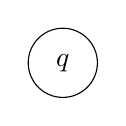
\begin{tikzpicture}[inner sep=1pt]
   \node[state] (A) {$q$};
\end{tikzpicture}

\hspace*{0.4cm} A beginning state is represented as $\rightarrow$
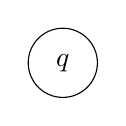
\begin{tikzpicture}[inner sep=1pt]
   \node[state] (A) {$q$};
\end{tikzpicture}


\hspace*{0.4cm} A final state is represented as
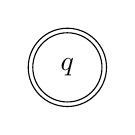
\begin{tikzpicture}[inner sep=1pt]
   \node[state] (A) {$q$};
   \node[state,inner sep=10pt]  (B) {$$};
\end{tikzpicture}

\vspace*{0.2cm}
\hspace*{0.4cm} An FA is represented in graphical format in Fig. 3.3.\\

\begin{center}
\section{picture}
\includegraphics[width=8cm,height=4cm]{50-2.png}
\end{center}

\newpage
\begin{flushright}
 \texttt{Finite Automata} \hspace*{1cm} \textbf{51}
\end{flushright}

\vspace*{0.2cm}
\textbf{Here}\\
\hspace*{1.5cm} $Q : \{q_{0}, q_{1}, q_{2}\}$ \\
\hspace*{1.5cm} $\Sigma : \{a, b\}$ \\
\hspace*{1.5cm} $\delta : \delta(q_{0}, a) \rightarrow q1$ \\
\hspace*{2cm} $\delta(q_{0}, b) \rightarrow q_{2}$ \\
\hspace*{2cm} $\delta(q_{1}, a) \rightarrow q_{0}$ \\
\hspace*{2cm} $\delta(q_{1}, b) \rightarrow q_{2}$ \\
\hspace*{2cm} $\delta(q_{2}, a) \rightarrow q_{2}$ \\
\hspace*{2cm} $\delta(q_{2}, b) \rightarrow q_{1}$ \\
\hspace*{1.5cm} $q_{0} : \{q_{0}\}$ \\
\hspace*{1.5cm} $F : \{q_{2}\}$ \\

\vspace*{0.2cm}
2. In the tabular format, a state is represented by the name of the state.\\
The beginning state is represented as $\rightarrow q_{n}$ \\

\hspace*{0.4cm} The final state is represented as
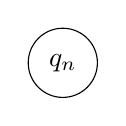
\begin{tikzpicture}[inner sep=1pt]
   \node[state] (A) {$q_{n}$};
\end{tikzpicture}

\vspace*{0.3cm}
\begin{center}
\section{picture}
\includegraphics[width=6cm,height=3.5cm]{51.png}
\end{center}


\vspace*{0.2cm}
\textbf{Here}\\
\hspace*{1.5cm} $Q : \{q_{0}, q_{1}, q_{2}\}$ \\
\hspace*{1.5cm} $\Sigma : \{a, b\}$ \\
\hspace*{1.5cm} $\delta : \delta(q_{0}, a) \rightarrow q1$ \\
\hspace*{2cm} $\delta(q_{0}, b) \rightarrow q_{2}$ \\
\hspace*{2cm} $\delta(q_{1}, a) \rightarrow q_{0}$ \\
\hspace*{2cm} $\delta(q_{1}, b) \rightarrow q_{2}$ \\
\hspace*{2cm} $\delta(q_{2}, a) \rightarrow q_{2}$ \\
\hspace*{2cm} $\delta(q_{2}, b) \rightarrow q_{1}$ \\
\hspace*{1.5cm} $q_{0} : \{q_{0}\}$ \\
\hspace*{1.5cm} $F : \{q_{2}\}$ \\

\vspace*{0.1cm}
\large{
\textbf{3.6 Transitional System}\\
}

\vspace*{0.2cm}

A transitional system (sometimes called the transitional graph) is a finite-directed graph in which each
node (or vertex) represents a state, and the directed arc indicates the transition of the state. The label of
the arc indicates the input or output or both.\\
\hspace*{0.5cm} A transitional function has two properties.\\

\vspace*{0.1cm}
\begin{enumerate}
  \item \textbf{Property I:} $\delta(q, \Lambda) \rightarrow q.$ It means if the input is given null for a state, the machine remains in the
same state.\\
\end{enumerate}


\newpage
 \begin{flushleft}
    \textbf{50}\hspace*{0.1cm} \textbf{$|$} \hspace*{0.1cm} Introduction to Automata Theory, Formal Languages and Computation
  \end{flushleft}
\vspace*{0.3cm}

\fcolorbox{blue}{blue}{\textcolor[rgb]{1.00,1.00,1.00}{2}} \textbf{Property II:} For all string $X$ and input symbol $a \varepsilon \Sigma$,\\
\begin{center}
  $\delta(q, Xa) \rightarrow \delta(\delta(q, X), a)$ \\
  $\delta(q, aX) \rightarrow \delta(\delta(q, a), X)$ \\
\end{center}
\vspace*{0.1cm}

\large{
\textbf{3.6.1 Acceptance of a String by Finite Automata}\\
}
\vspace*{0.2cm}


There are two conditions for declaring a string to be accepted by a finite automaton. The conditions are\\

\vspace*{0.2cm}
\hspace*{0.5cm} \textbf{Condition I:} The string must be totally traversed.\\

\hspace*{0.5cm} \textbf{Condition II:} The machine must come to a final state.\\

\vspace*{0.2cm}

In short, it can be said that if $\delta(q_{0}, W) = q_{n}$, where W is the string given as input to the FA, $q_{0}$ is the beginning
state, and $q_{n}$ belongs to the set of final states, then the string W can be said to be accepted by the FA.\\
\hspace*{0.5cm} If these two conditions are fulfilled, then we can declare a string to be accepted by an FA.\\


\hspace*{0.5cm} If any of the conditions are not fulfilled, then we can declare a string to be not accepted by an FA.\\
\hspace*{0.5cm} The following examples (Examples 3.1 and 3.2) describe this.\\

\fcolorbox{red}{blue}{\textbf{\textcolor[rgb]{1.00,1.00,1.00}{Example 3.1}}}\hspace*{0.1cm} Check whether the string 011001 is accepted or not by the following FA.\\
\vspace*{0.1cm}

\begin{center}
\section{picture}
\includegraphics[width=5.5cm,height=3.5cm]{52.png}
\end{center}

\vspace*{0.1cm}

\textbf{Solution:} For the given FA, $Q = \{q_{0}, q_{1}, q_{2}, q_{3}\} \Sigma = \{0, 1\}$. The beginning state is $q_{0}$ and the final state
is $_{q}$.\\

\hspace*{0.5cm} The transitional functions are given in the table.\\
\hspace*{0.5cm} For checking whether a string is accepted by an FA or not, we will assume that the input string is
given input in the beginning state q0. But only a single input is given in each clock pulse. So, at first,
the left most character is given the input to the beginning state. From the transitional function given in
the table, the next state is determined. The next character of the input string is treated as the input to the
state just achieved. And it will process like this till the string is fi nished or such a condition has arrived
so that there is no transitional function mentioned in the table.\\
\hspace*{0.5cm} If the string is finished and the state achieved is the final state, then the string will be declared
accepted by the machine.\\
\hspace*{0.5cm} If it does not happen, then the string will be declared not accepted.\\
\hspace*{3.4cm} $\delta(q0, 011001) \rightarrow \delta(q_{0}, 11001)$ \\
\hspace*{5cm} $\rightarrow \delta(q_{1}, 1001)$ \\
\hspace*{5cm} $\rightarrow \delta(q_{3}, 001)$ \\
\hspace*{5cm} $\rightarrow \delta(q_{1}, 01)$ \\
\hspace*{5cm} $\rightarrow \delta(q_{2}, 1)$ \\
\hspace*{5cm} $\rightarrow q_{3}$ \\

\end{document} 